\begin{frame}{}
    \begin{center}
        \LARGE An\'alisis
    \end{center}
\end{frame}


\begin{frame}{Estrategia del an\'alisis de datos}
\begin{itemize}
\item El an\'alisis se basa en una selecci\'on de eventos a partir de una serie de variables experimentales las cuales buscan optimizar la eficiencia de la se\~nal y reducir lo mas posible los procesos de ruido.
\item Recordar que en los datos experimentales solo se tiene informaci\'on de los muones reconstruidos y a partir de eso se infiere la posible producci\'on de fotones oscuros.
\item La selecci\'on de eventos se aplica a cada una de las muestras de simulaci\'on generadas y se estudia las eficiencias y distribuciones caracter\'isticas.
\end{itemize}    
\end{frame}


\begin{frame}{Secuencia del an\'alisis de datos}

\begin{itemize}
    \item El an\'alisis comienza con la muestra simulada (raw data) 
    \item Se procede a la selecci\'on de eventos, donde se reduce la cantidad de datos a analizar 
    \item Se procede a la obtenci\'on de resultados, gracias estad\'isticas y discusi\'on de los mismos, algo similar al esquema mostrado en la figura 
\end{itemize}


\begin{figure}[h]
\centering
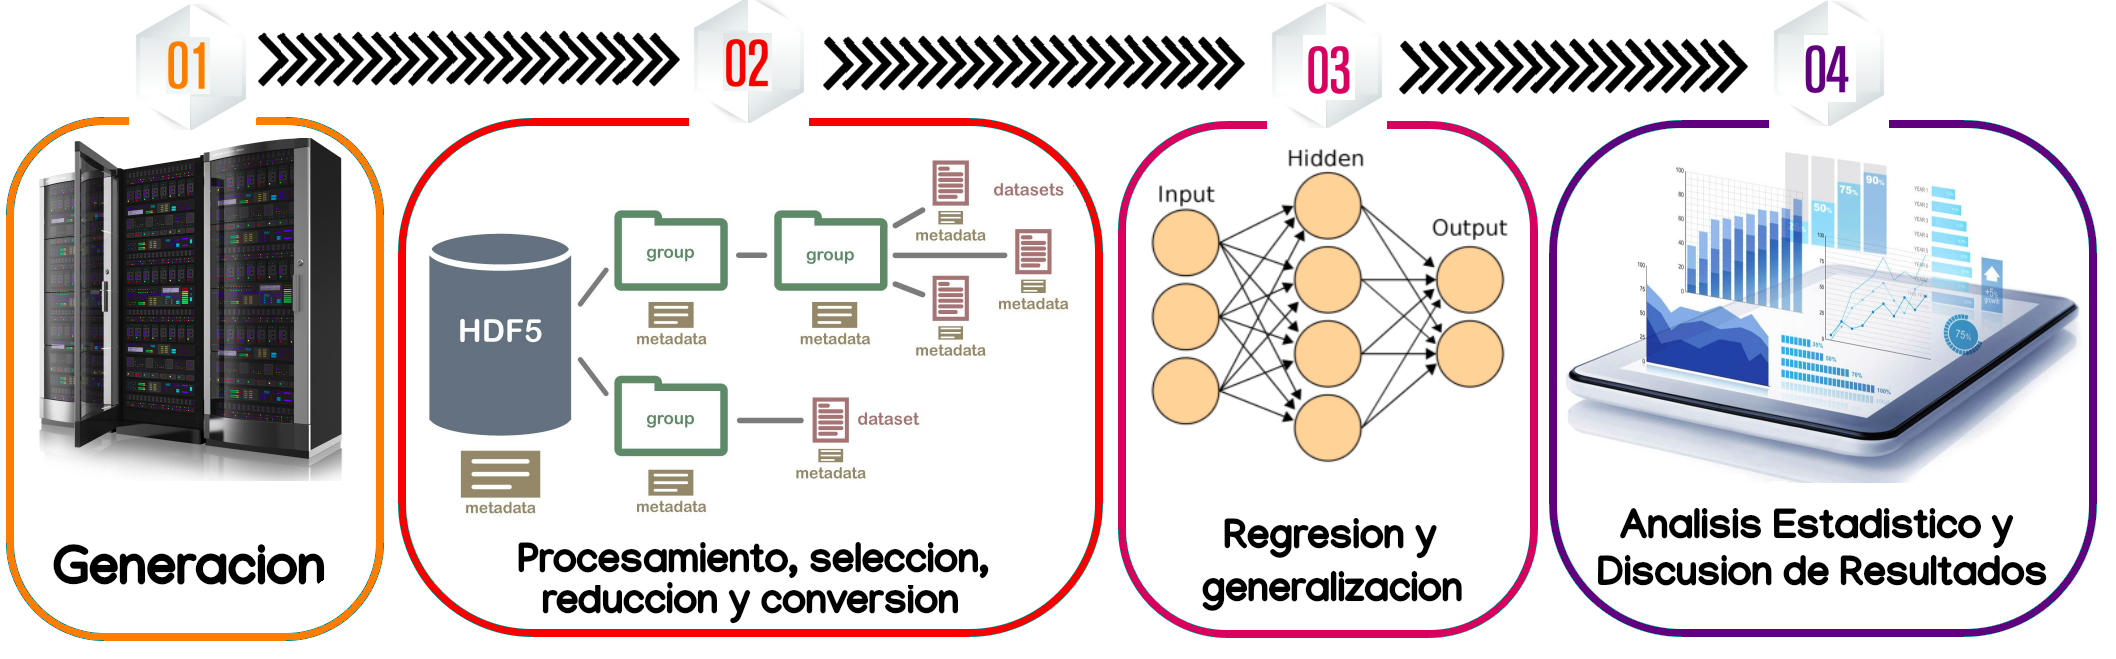
\includegraphics[width=0.8\textwidth]{Imag/procesos_darksusy.png}
\caption{Secuencia del an\'alisis de datos}
\end{figure}

\end{frame}


\begin{frame}{Estructura del c\'odigo de an\'alisis}

\begin{itemize}
    \item Se desarrollo un entorno de simulaci\'on y an\'alisis de datos el cual esta basado en c\'odigo de python y ROOT. 
    \item El entorno se encuentra hospedado en ACARUS y puede ser f\'acilmente extendido para el an\'alisis de otros modelos (adicionales a Dark-SUSY)
\end{itemize}
    
\begin{figure}[h]
\centering
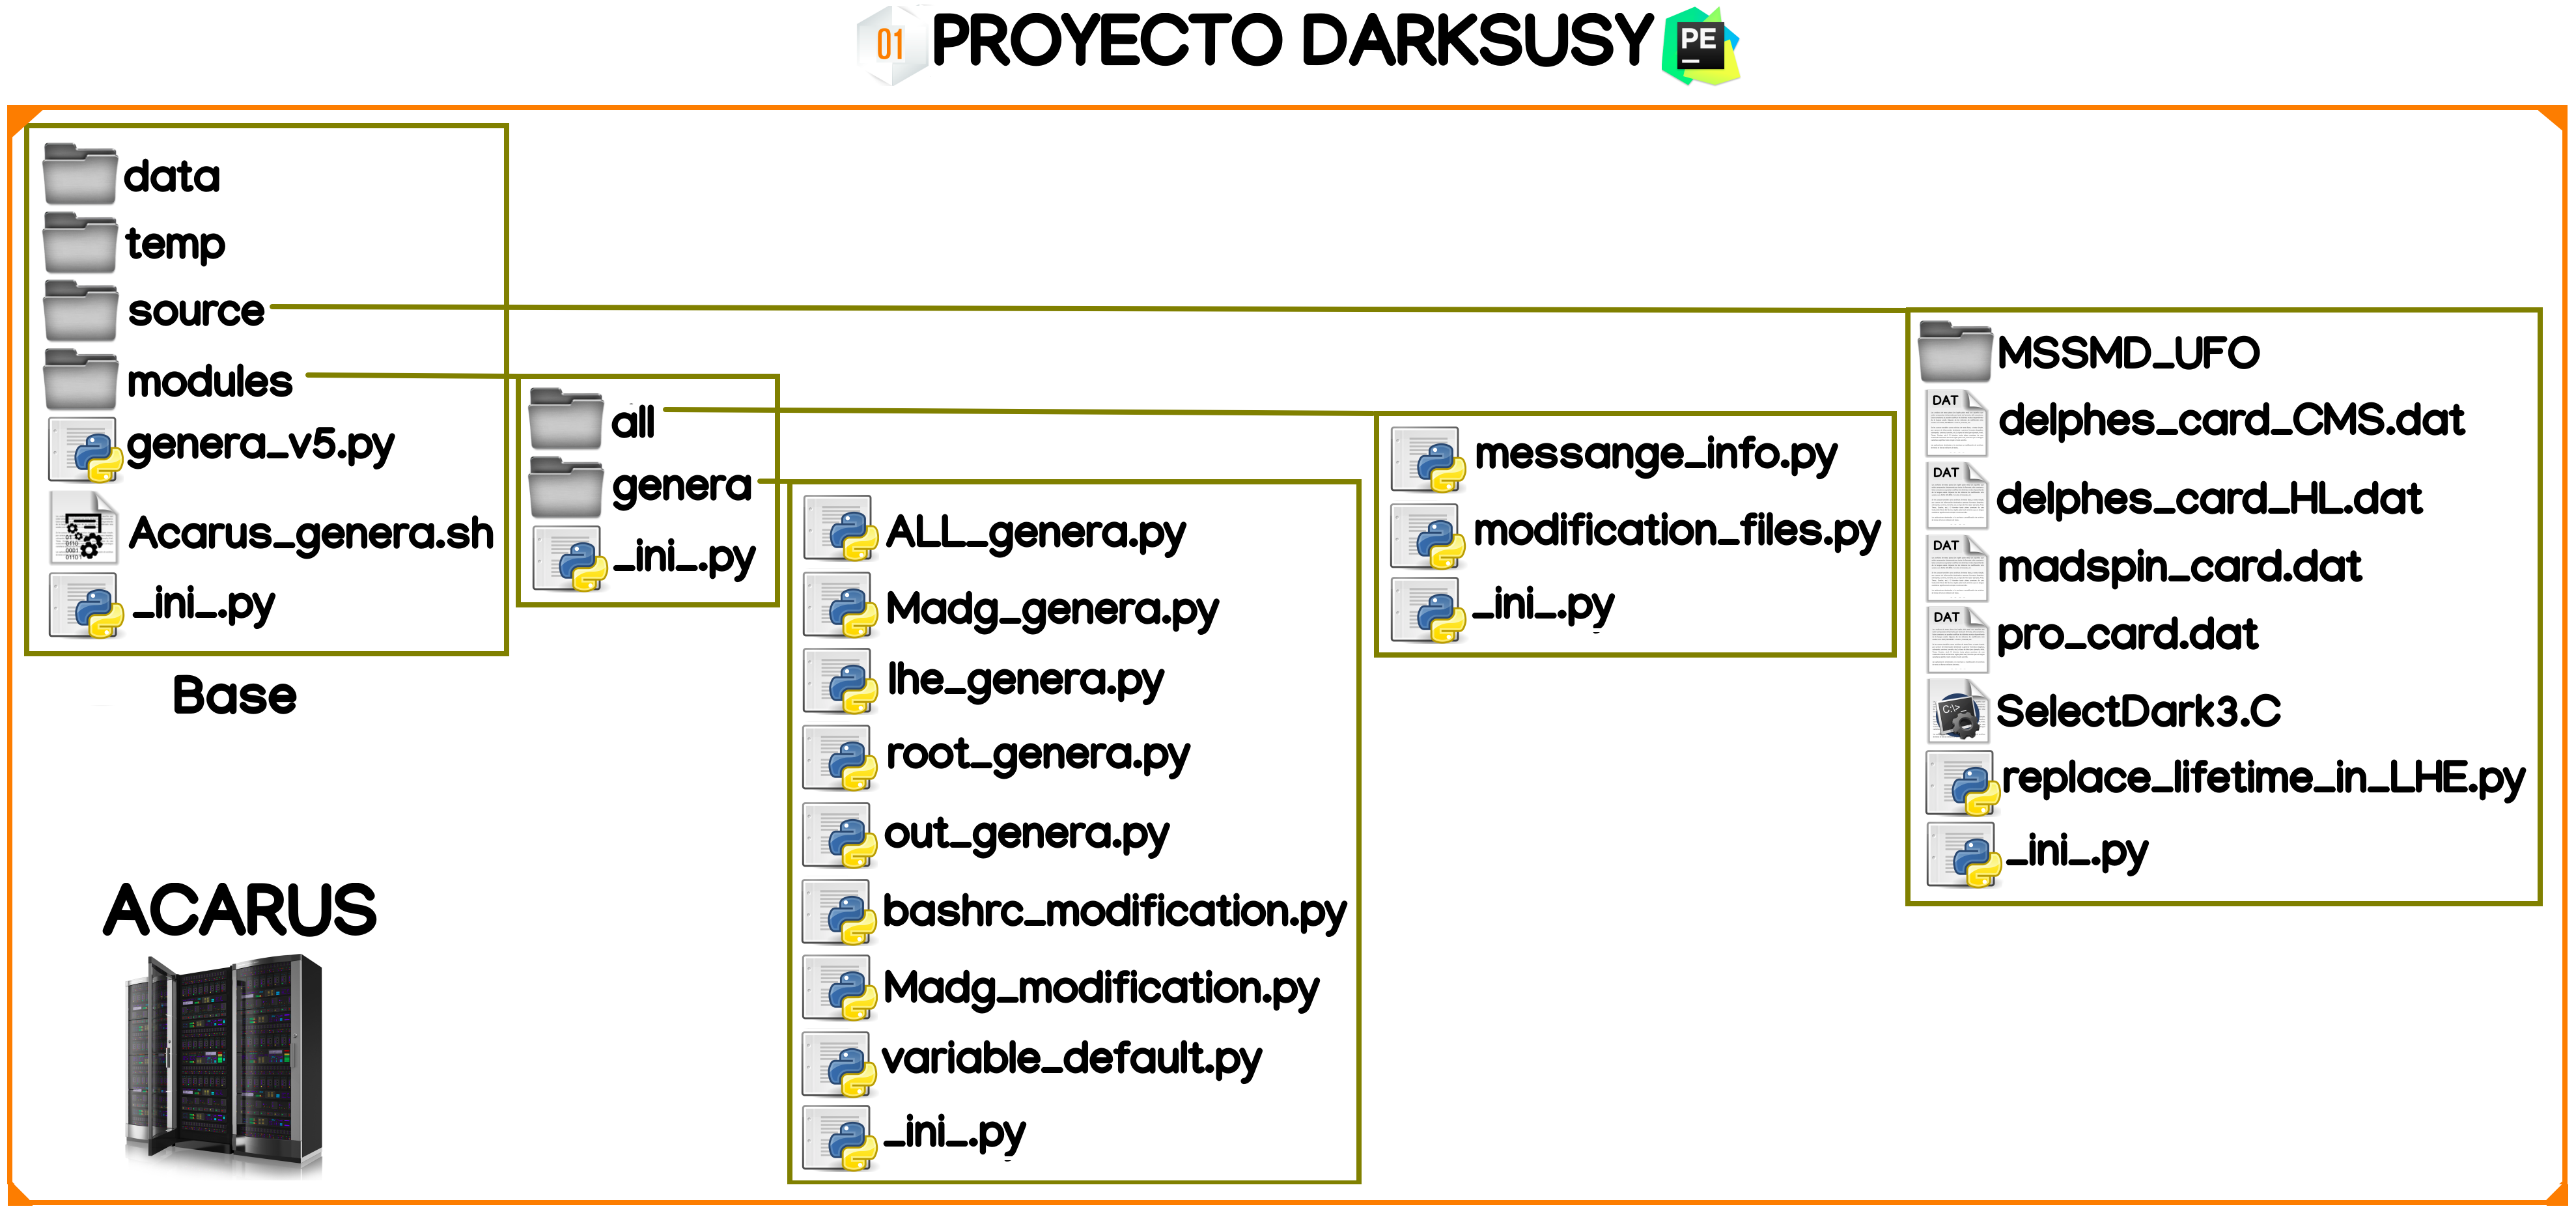
\includegraphics[width=0.8\textwidth]{Imag/proyecto_darksusy.png}
\caption{Estructura del c\'odigo de an\'alisis}
\end{figure}

\end{frame}



\begin{frame}{Selecci\'on preliminar}

\begin{itemize}
%\item \textbf{4$\mu$}: Selecci\'on de eventos con al menos 4 muones
%	\begin{itemize}
%		\item Muones con un momento transversal ($p_{T}$) mayor a
%		\item Muones con un valor de pseudo-rapidez ($|\eta|$) menor a 2.4
%	\end{itemize}
\item \textbf{Algoritmo de pariamiento de muones}: Encontrar el par de muones \'optimos que con mayor probabilidad podr\'ian ser generados por un fot\'on oscuro.

\item \textbf{Algoritmo con identificador de machine learning di-muon}: Optimizas la detecci\'on haciendo conocida las muestras y pareamientos reales con la paqueter\'ia de tensorflow.

\end{itemize}
    
\end{frame}


\begin{frame}{Algoritmo de pariamiento de muones}
% \color{red} Francisco aqui incluir el diagrama de algoritmo de pariamiento
\begin{figure}[h]
\centering
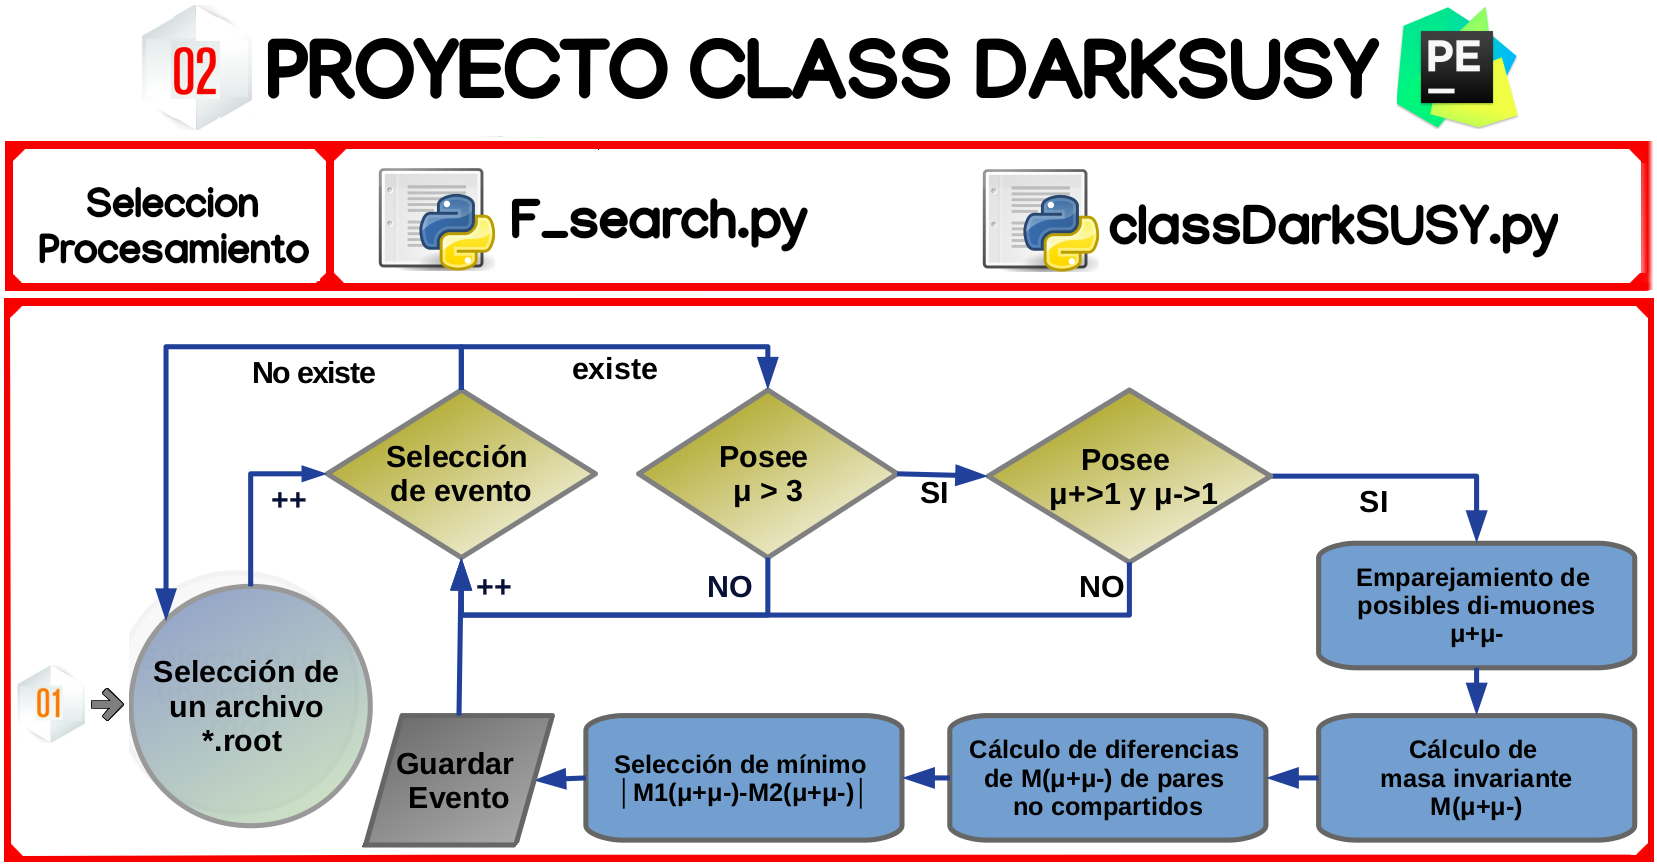
\includegraphics[width=1\textwidth]{Imag/class_darksusy.png}
\caption{Diagrama de algoritmo de pariamiento. Eficiencia conocida de 87\%.}
\end{figure}   
\end{frame}


\begin{frame}{Algoritmo con identificador de machine learning di-muon}
Proceso de entrenamiento y creaci\'on del modelo.
\begin{figure}[h]
\centering
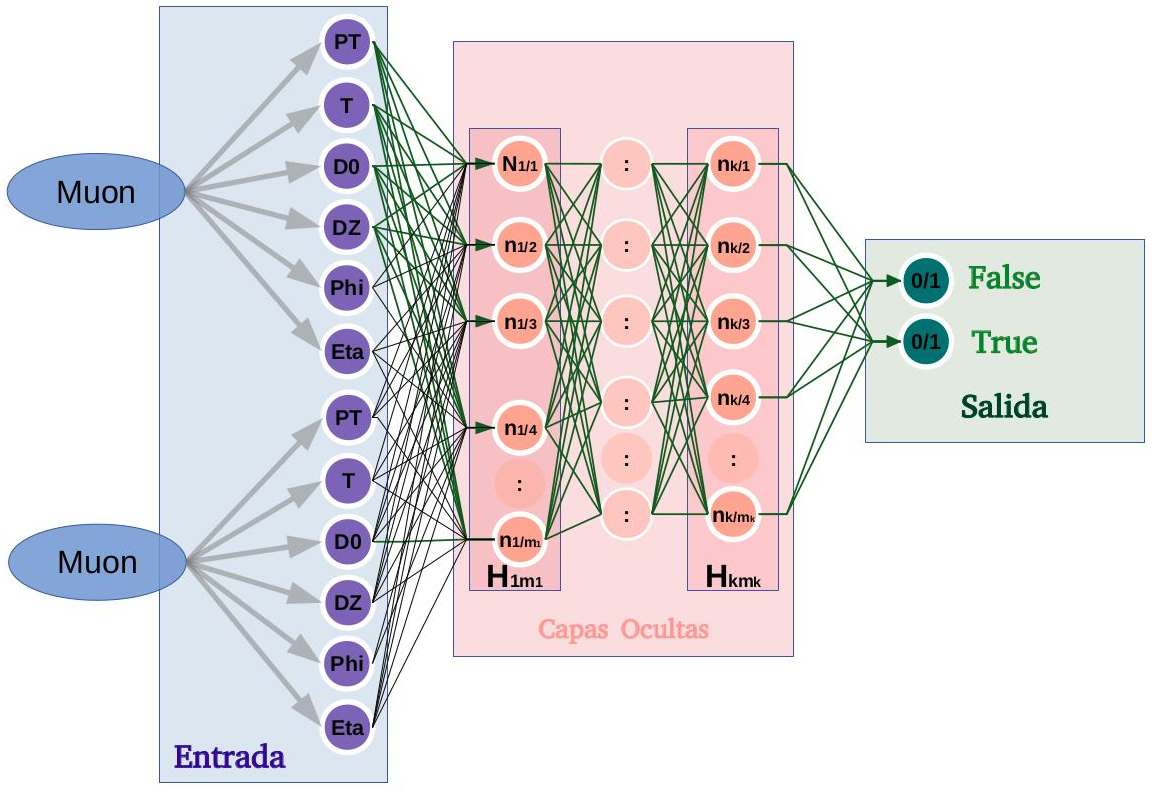
\includegraphics[width=.8\textwidth]{Imag/IDENTIFICADOR.png}
\caption{Creaci\'on del identificador. Eficiencia conocida de 98\%.}
\end{figure}   
\end{frame}


\begin{frame}{Eficiencia para fot\'on oscuro con detector CMS}
\begin{small}
%\color{red} Francisco llenar estos numeros \color{black}
\begin{table}[]
\centering
\begin{tabular}{c|c|c|c|c|c|}
Selecci\'on  & $c\tau=0.5$ & $c\tau=5$ & $c\tau=10$ & $c\tau=50$ & $c\tau=100$ \\  \hline
Sin corte    &  10 000 & 10 000 & 10 000 & 10 000 & 10 000\\
4-$\mu$      &  916 & 500 & 227 & 16 & 2 \\
pariamiento  &  916 & 500 & 227 & 16 & 2
\end{tabular}
\caption{Tabla con el numero de eventos despu\'es de cada selecci\'on $m_{\gamma_{D}}$=0.25 GeV y diferentes valores del tiempo de vida para el detector CMS.}
\end{table}

\begin{table}[h]
\centering
\begin{tabular}{c|c|c|c|c|c|}
Selecci\'on  & $c\tau=0.5$ & $c\tau=5$ & $c\tau=10$ & $c\tau=50$ & $c\tau=100$ \\ \hline
Sin corte   & 10 000 & 10 000 & 10 000 & 10 000 & 10 000\\
4-$\mu$     & 955 & 968 & 947 & 862 & 655 \\
pariamiento & 955 & 968 & 947 & 862 & 655
\end{tabular}
\caption{Tabla con el n\'umero de eventos despu\'es de cada selecci\'on $m_{\gamma_{D}}~=~ 8~GeV$ y diferentes valores del tiempo de vida para el detector CMS.}
\end{table}

\end{small}

\end{frame}



\begin{frame}{Distribuciones caracter\'isticas: Masa invariante}
    
\begin{itemize}
\item Despu\'es de la selecci\'on preliminar se puede reconstruir la masa de los muones, dicha masa corresponder\'ia a la masa de los fotones oscuros. A continuaci\'on se muestra un ejemplo para los procesos con un valor esperado de $m_\gamma = 4 GeV$: 
\end{itemize}
    
\begin{figure}[ht]
\centering
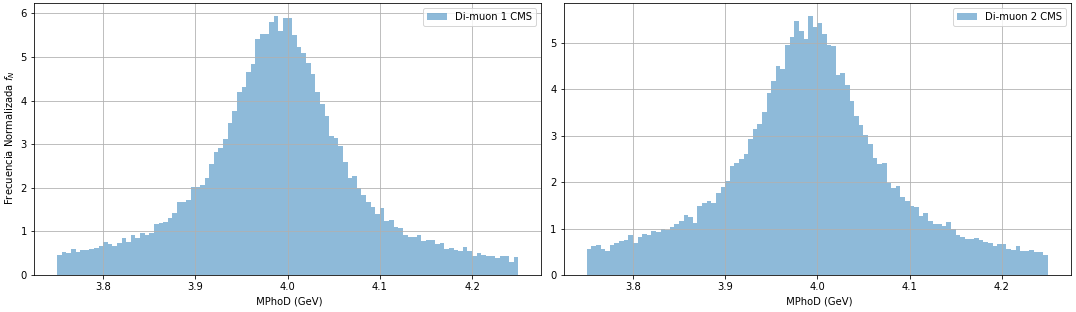
\includegraphics[width=1\textwidth]{Imag/Datos_Photon4muon_CORTE_CMS.png}
\caption{Masa invariante para los di-muones.}
\end{figure}
%\begin{figure}[ht]
%\begin{minipage}[b]{0.45\linewidth}
%\centering
%
\includegraphics[width=1\textwidth]{Imag/placeholder.png}
%\caption{Masa invariante primer di-muon}
%\end{minipage}
%\hspace{0.5cm}
%\begin{minipage}[b]{0.45\linewidth}
%\centering
%
\includegraphics[width=1\textwidth]{Imag/placeholder.png}
%\caption{Masa invariantes segundo di-muon}
%\end{minipage}
%\end{figure}
\end{frame}



\begin{frame}{Distribuciones caracter\'isticas: Par\'ametros}

\begin{figure}[h]
\centering
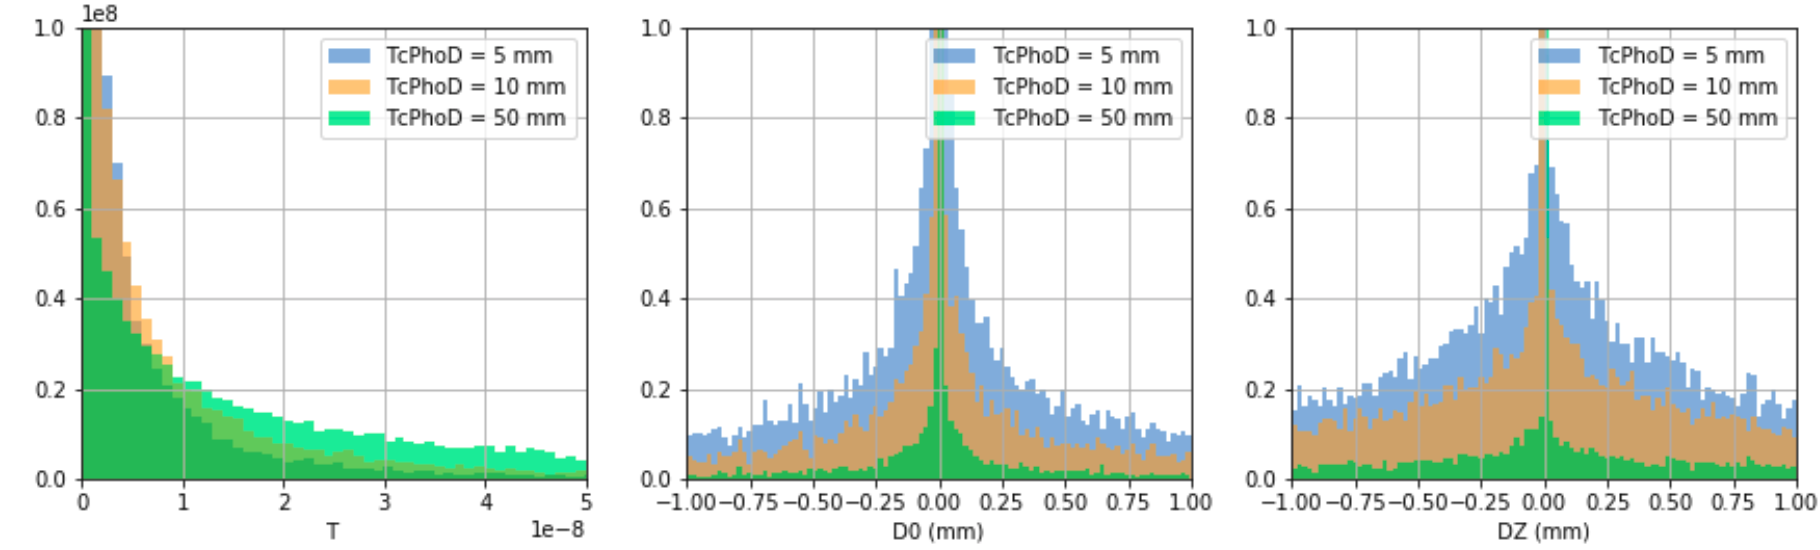
\includegraphics[width=1\textwidth]{Imag/variar_parametros.png}
\caption{Variaciones de algunas propiedades del muon con el cambio de tiempo de vida del f\'oton oscuro.}
\end{figure} 

\end{frame}


\begin{frame}{}
    \begin{center}
        \LARGE High Luminosity LHC
    \end{center}
\end{frame}


\begin{frame}{Eficiencia para fot\'on oscuro para detector HL.}
\begin{small}
%\color{red} Francisco llenar estos numeros \color{black}
\begin{table}[]
\centering
\begin{tabular}{c|c|c|c|c|c|}
Selecci\'on  & $c\tau=0.5$ & $c\tau=5$ & $c\tau=10$ & $c\tau=50$ & $c\tau=100$ \\  \hline
Sin corte    &  10 000 & 10 000 & 10 000 & 10 000 & 10 000\\
4-$\mu$      &  1678 & 902 & 433 & 39 & 6 \\
pariamiento  &  1678 & 902 & 433 & 39 & 6
\end{tabular}
\caption{Tabla con el n\'umero de eventos despu\'es de cada selecci\'on $m_{\gamma_{D}}$=0.25 GeV y diferentes valores del tiempo de vida para el detector HL.}
\end{table}

\begin{table}[h]
\centering
\begin{tabular}{c|c|c|c|c|c|}
Selecci\'on  & $c\tau=0.5$ & $c\tau=5$ & $c\tau=10$ & $c\tau=50$ & $c\tau=100$ \\ \hline
Sin corte   & 10 000 & 10 000 & 10 000 & 10 000 & 10 000\\
4-$\mu$     & 1914 & 1915 & 1844 & 1614 & 1208 \\
pariamiento & 1914 & 1915 & 1844 & 1614 & 1208
\end{tabular}
\caption{Tabla con el n\'umero de eventos despu\'es de cada selecci\'on $m_{\gamma_{D}}~=~ 8~GeV$ y diferentes valores del tiempo de vida para el detector HL.}
\end{table}
\end{small}
\end{frame}

\begin{frame}{Eficiencia para fot\'on oscuro. Regresi\'on.}
Con la intenci\'on de generalizar los valores de eficiencia de los detectores  mediante un m\'etodo predictivo, se intenta aplicar dos m\'etodos de regresi\'on : \\
1- M\'etodo de regresi\'on Polinomial
\begin{equation}
\ln y = \sum_{i=0}^k (\alpha_{0i} + \alpha_{1i}\cdot x_i + \alpha_{2i}\cdot x_i^2 + \alpha_{3i}\cdot x_i^3 + \ldots+\alpha_{ni} \cdot x_i^n)+\epsilon
\end{equation}
el orden de la regresi\'on est\'a dado por $n$ y los valores $x_i$ ser\'an las variables independientes de nuestro modelo, estos fueron integrados en una funci\'on en python implementando la paqueteria sklearn con la flexibilidad de cambiar los valores $k$ y $n$.

\end{frame}

\begin{frame}{Eficiencia para fot\'on oscuro. Regresi\'on.}
Los resultados de su implementaci\'on de la regresi\'on polinomial:\\
1- M\'etodo de regresi\'on Polinomial

\begin{figure}
\centering
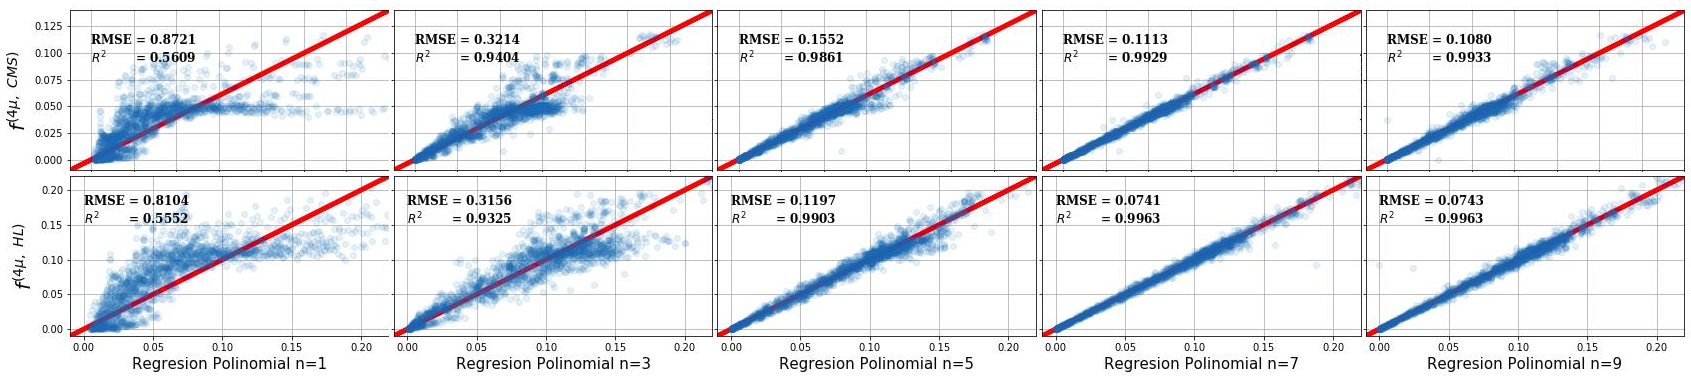
\includegraphics[width=1\textwidth]{Imag/regresionlineal.png}
\caption{Resultados del ajuste de correlaci\'on para la regresi\'on polinomial.}
\end{figure}
\end{frame}



\begin{frame}{Eficiencia para fot\'on oscuro. Regresi\'on.}
2- M\'etodo de regresi\'on con machine learning, aplicaci\'on m\'odulo keras:\\
\begin{figure}
\centering
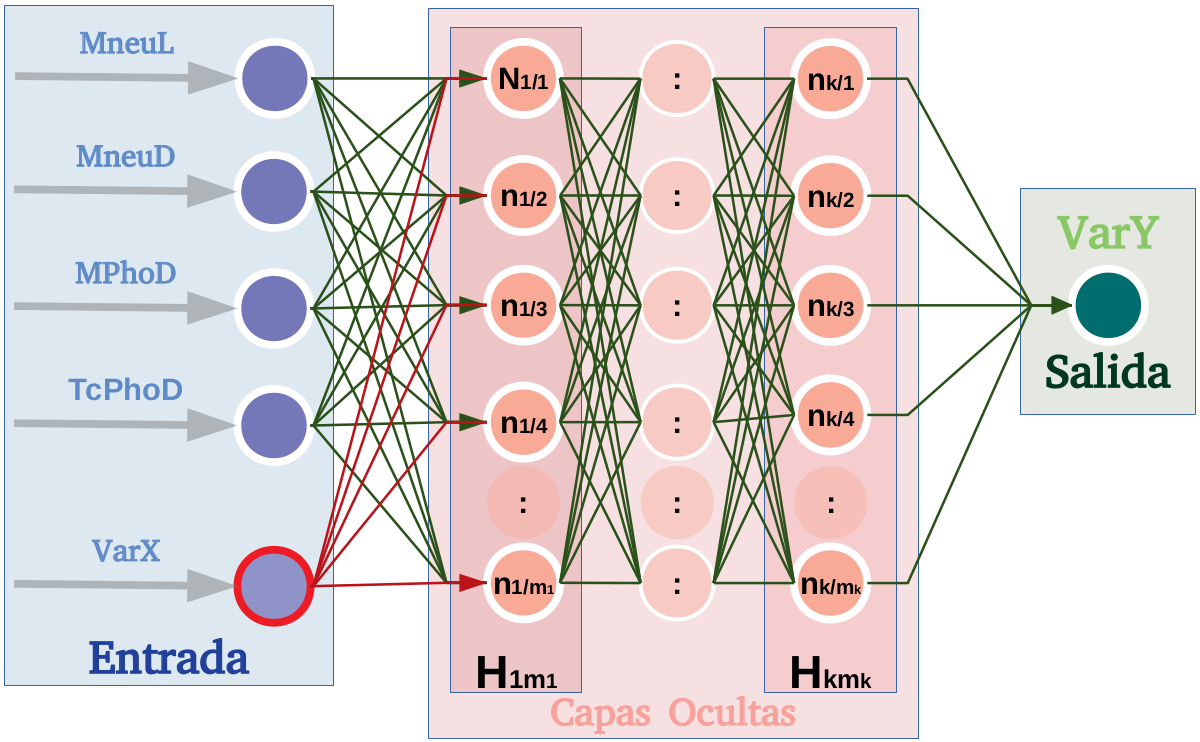
\includegraphics[width=.6\textwidth]{Imag/neuronas.png}
\caption{Diagrama de la estructura general de la red neuronal.}
\end{figure}
Para el caso de las eficiencias (VarY) este diagrama se adapta a 4 neuronas de entrada sin la variable VarX que es opcional. 
\end{frame}


\begin{frame}{Eficiencia para fot\'on oscuro. Regresi\'on.}
2- M\'etodo de regresi\'on con machine learning, aplicaci\'on m\'odulo keras:\\
Resultados y comparaci\'on:
\begin{figure}
\centering
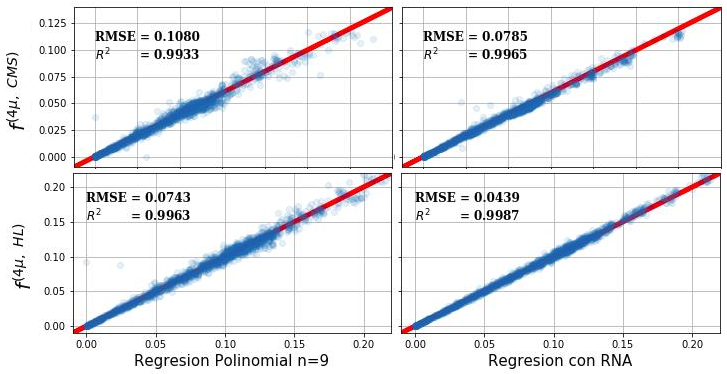
\includegraphics[width=1\textwidth]{Imag/regresion2.png}
\caption{Comparaci\'on entre los m\'etodos de regresi\'on.}
\end{figure}

\end{frame}


\begin{frame}{Etapa de Alta luminosidad para el Gran Colisionador de Hadrones}
    \begin{itemize}
        \item El Gran Colisionador de Hadrones junto con sus experimentos principales estan en una etapa de actualizacion en preparacion para la etapa de alta luminosidad (2025-2035) 
        \item En particular para la deteccion de muones se instalaran una serie de nuevos detectores que ampliaran el rango de deteccion, muy en particular para la region de pseudo-rapidez ($2.4<|\eta|<3.0$) como se muestra en el la imagen
        \item Estos nuevos detectores permitiran la identificacion de muones en esta region, y aumentaran la probabilidad de detectar se\~nales como los fotones oscuros
    \end{itemize}
\end{frame}



\begin{frame}{Actualizaci\'on del sistema de muones en el HL-LHC}

\begin{itemize}
\item La actualizaci\'on de basa en la instalaci\'on de nuevos detectores de muones 
\item Dicha detecci\'on amplia el rango de b\'usqueda para la posible detecci\'on de muones provenientes del fot\'on oscuro y otros modelos de fisica mas alla del modelo est\'andar
\end{itemize}

\begin{figure}
\centering
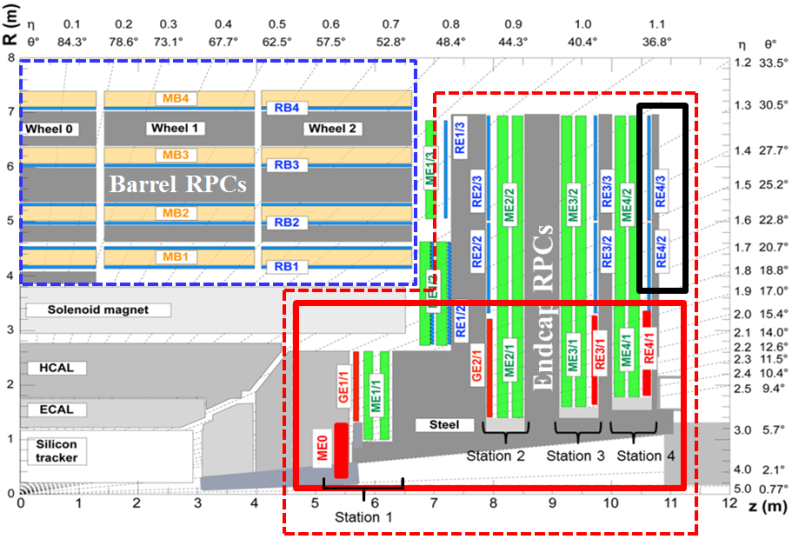
\includegraphics[width=.6\textwidth]{Imag/muon_phase-2.png}
\caption{Actualizaci\'on del sistema de muones para la fase de alta luminosidad.}
\end{figure}

\end{frame}


\begin{frame}{Comparacion distribuciones detector actual vs HL-LHC}
%\color{red} Francisco aqui poner distribucion de pseudorapidez comparando el detector actual y el detector nuevo
\begin{figure}
\centering
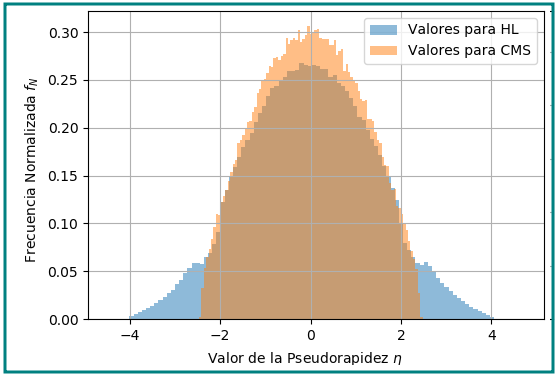
\includegraphics[width=.8\textwidth]{Imag/Datos_Eta_ALL_simple.png}
\caption{Comparar pseudorapidez.}
\end{figure}  
\end{frame}

\begin{frame}{Comparacion distribuciones detector actual vs HL-LHC}
\begin{figure}
\centering
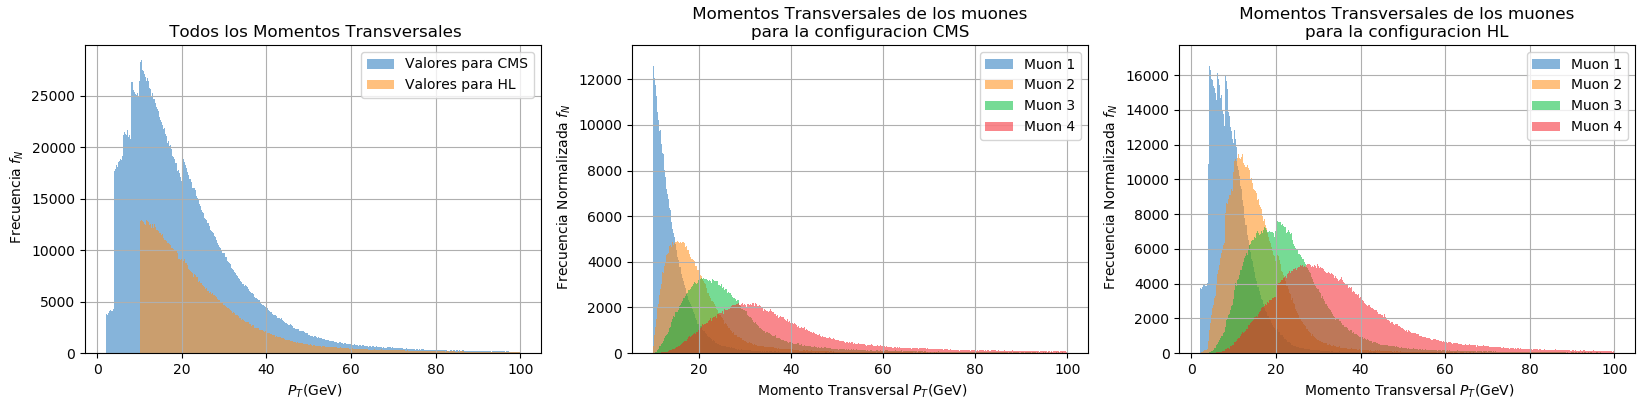
\includegraphics[width=1\textwidth]{Imag/momento1.png}
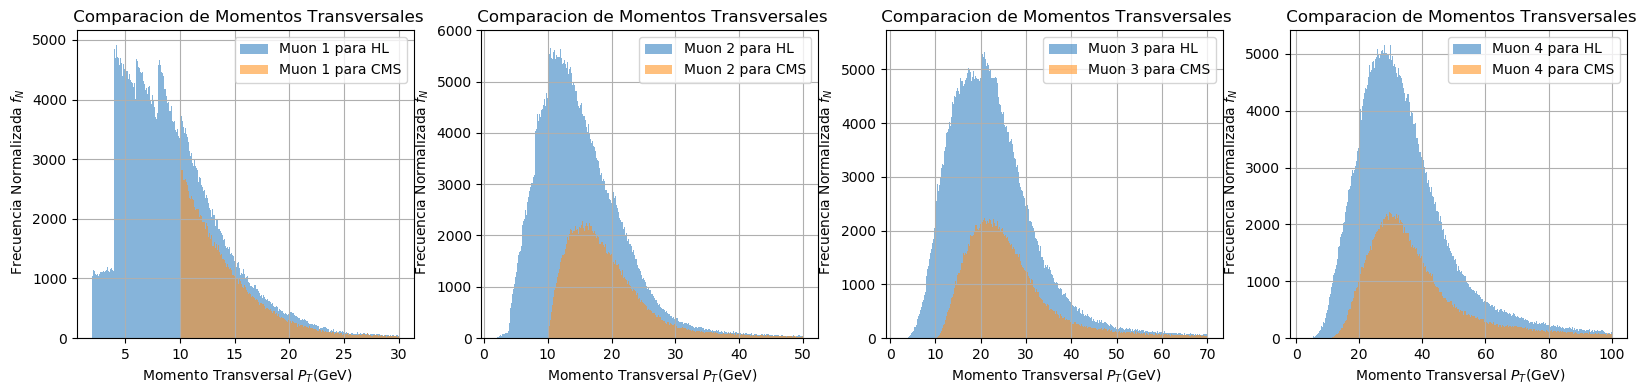
\includegraphics[width=1\textwidth]{Imag/momento2.png}
\caption{Comparar momentos.}
\end{figure}  
\end{frame}



\begin{frame}{Comparaci\'on de eficiencias detector actual vs HL-LHC.}
    
\begin{itemize}
\item Las ventajas de las actualizaciones se ve reflejada como una aumento en la eficiencia de la se\~nal
\item La b\'usqueda del fot\'on oscuro durante el HL-LHC es uno de los objetivos fundamentales
\end{itemize}
    
\begin{figure}[h]
\centering
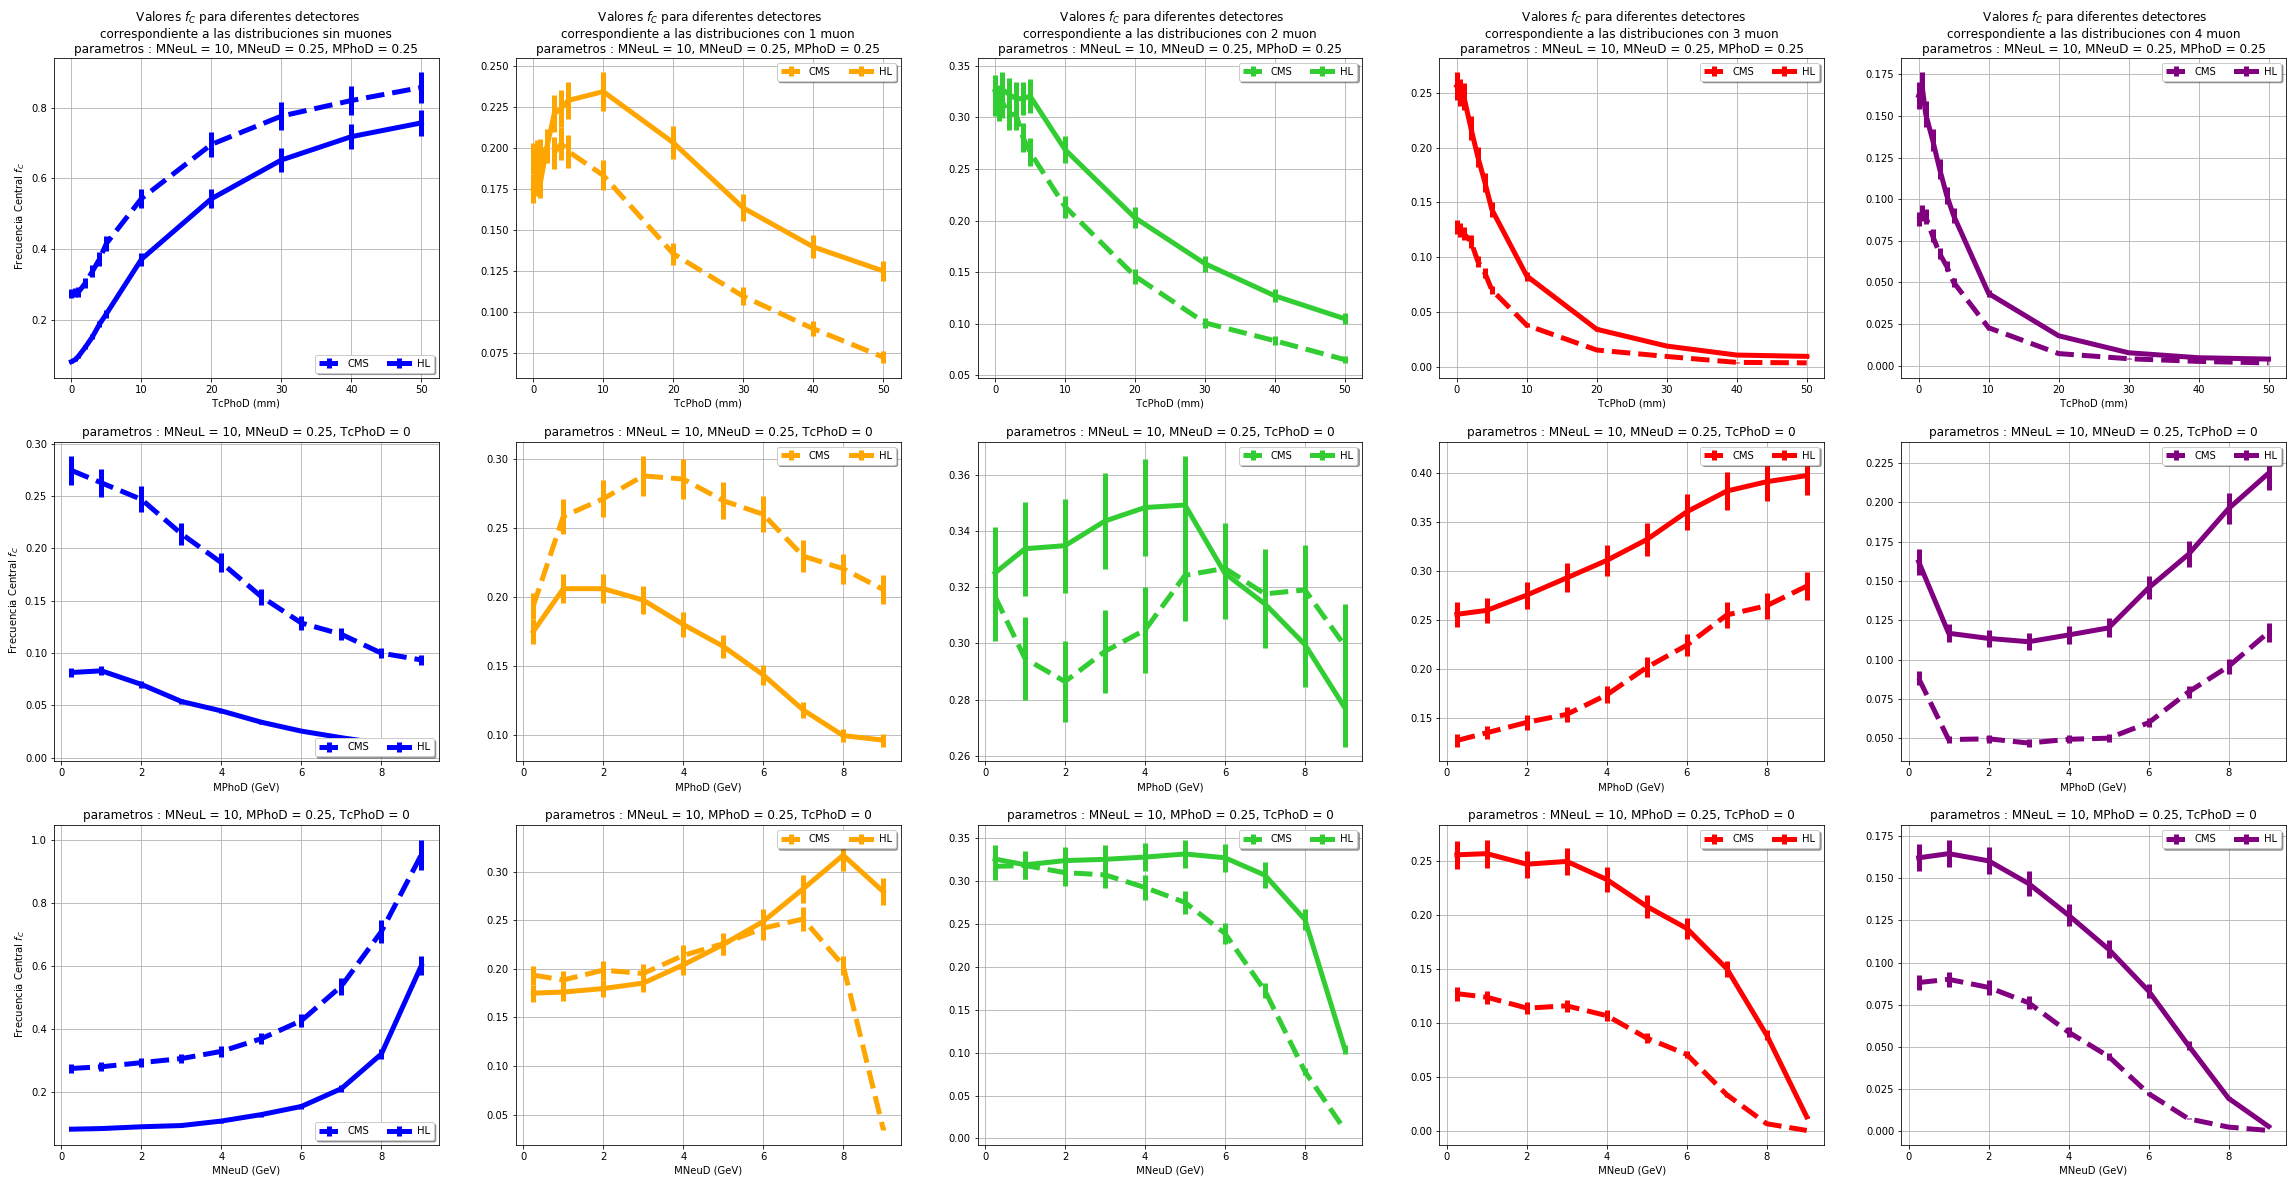
\includegraphics[width=0.7\textwidth]{Imag/Comparacion_Distribucion_Entries.png}
\caption{Comparaci\'on de eficiencias del detector actual vs HL-LHC para las diferentes muestras}
\end{figure}

\end{frame}


\begin{frame}{Comparaci\'on de eficiencias detector actual vs HL-LHC.}

\begin{itemize}
\item se logr\'a una mejor estimaci\'on de la masa.
\end{itemize}
\begin{figure}[h]
\centering
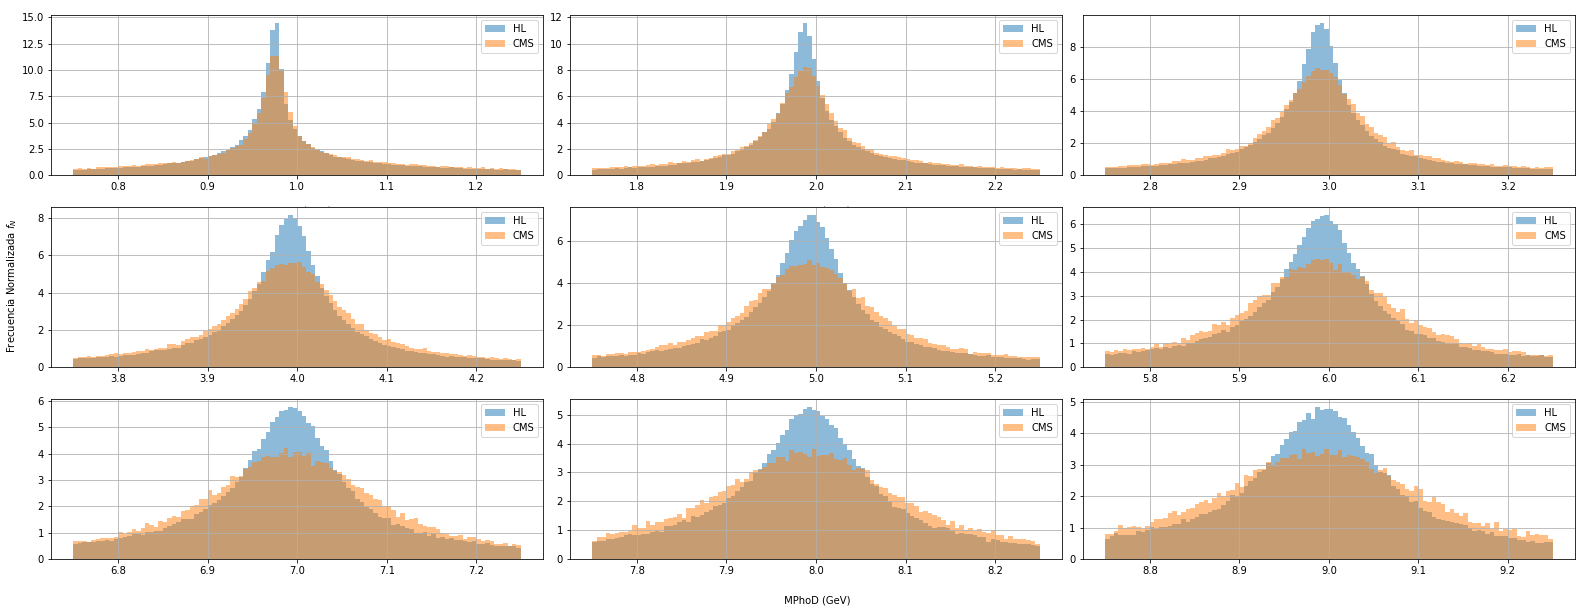
\includegraphics[width=1\textwidth]{Imag/Datos_Photon4muon_ALL.png}
\caption{Comparaci\'on de la distribuci\'on normalizada de masas del fot\'on.}
\end{figure}
\end{frame}



\begin{frame}{Resumen}
\begin{itemize}
\item Se integro el modelo Dark-SUSY en un entorno de simulaci\'on
\item Se desarrollo un entorno de simulaci\'on y an\'alisis el cual usa los recursos computacionales de la Universidad de Sonora (ACARUS) para generar resultados 
\item Se estudio a detalle la se\~nal caracteristica de los fotones oscuros
\item Se compar\'o la mejora en cuanto a eficiencia y rango de busqueda en la reconstruccion de muones del detector actual respecto a la actualizaci\'on en la etapa de alta luminosidad (HL-LHC) concluyendo que se tendr\'a en general $\sim$ 80-150\% m\'as de reconstrucciones de inter\'es para el fot\'on oscuro y un $\sim$ 12-19\% menos de errores en los valores de masa del fot\'on reconstruidos. %\color{red} Francisco poner una estimacion de este numero XXX\% \color{black} 
%de eficiencia en la b\'usqueda de esta se\~nal
\end{itemize}
  
\end{frame}



\begin{frame}{Siguientes Pasos}
\begin{itemize}
\item Finalizar escritura de tesis (Finales de Junio) 
\item Distribuir primer draft a  principios de Julio
\item Presentar a finales de Julio o principios de Agosto
\end{itemize}
    
\end{frame}